\documentclass{article}

\usepackage{stmaryrd}
\usepackage{amsmath}
\usepackage{amssymb}
\usepackage{amsthm}
\usepackage{relsize} 
\usepackage{bm} 
\usepackage{IEEEtrantools}
\usepackage{graphicx}
\usepackage{caption}
\usepackage{subcaption}
\usepackage{hyperref}
\usepackage{cases}
\usepackage{xfrac}
\usepackage{comment}
\usepackage{framed}
\usepackage{fancyhdr}
\usepackage{enumitem}
\usepackage{cite}
\usepackage[]{algorithm2e}
\usepackage[procnames]{listings}
\usepackage{color}
\usepackage[normalem]{ulem}

\definecolor{keywords}{RGB}{255,0,90}
\definecolor{comments}{RGB}{0,0,113}
\definecolor{red}{RGB}{160,0,0}
\definecolor{green}{RGB}{0,150,0}
 
\newcommand\pythonstyle{\lstset{language=Python, 
        basicstyle=\ttfamily\small, 
        keywordstyle=\color{keywords},
        commentstyle=\color{comments},
        stringstyle=\color{red},
        showstringspaces=false,
        identifierstyle=\color{green},
        procnamekeys={def,class}}}

\lstnewenvironment{python}[1][]
{
\pythonstyle
\lstset{#1}
}
{}

\newcommand\pythonexternal[2][]{{
\pythonstyle
\lstinputlisting[#1]{#2}}}

\oddsidemargin = 20pt
\textwidth = 420pt

\hypersetup{
     colorlinks   = true,
     linkcolor    = blue
}

\title{Project in Predictive Control and Real Time Systems}
\author{Marcus Greiff, Daniel Nilsson}
\begin{document}
\maketitle

\newpage
\tableofcontents
\newpage

\section{Introduction}
\section{Dynamics}
In this project, we consider the non-linear quadcopter equations as derived by Lukkonen et al. ~\cite{luukkonen2011modelling}. A brief description of the dynamics is given to define terms which will be used in the control scheme. Let
\begin{equation}
\boldsymbol{\xi} = \begin{bmatrix}x\\y\\z\end{bmatrix},\quad
\boldsymbol{\eta}= \begin{bmatrix}\phi\\\theta\\\psi\end{bmatrix},\quad
\boldsymbol{\omega}=\begin{bmatrix}\omega_1\\\omega_2\\\omega_3\\\omega_4\end{bmatrix},
\end{equation}
where $\boldsymbol{\xi}$ [m] denotes the position of the centre of mass in a global cartesian coordinate system, $\boldsymbol{\eta}$ [rad] is the euler-angles in the body coordinate system and $\omega_i$ [rad/s] is the angular speed of the rotor $i$. For future reference, the basis vectors in the cartesian coordinate system are written $\hat{\mathbf{\cdot}}$, and the subindexing $\mathbf{\cdot}_B$ refers to the vector of matrix defined in the body coordinate system.

The translation from the global- to the body coordinate system is done by the orthogonal rotation matrix
\begin{equation}
\mathbf{R} = 
\begin{bmatrix}
\cos(\psi)\cos(\phi) & \cos(\psi)\sin(\theta)\sin(\phi)- \sin(\psi)\cos(\phi) & \cos(\psi)\sin(\theta)\cos(\phi)+ \sin(\psi)\sin(\phi)\\
\sin(\psi)\cos(\phi) & \sin(\psi)\sin(\theta)\sin(\phi) + \cos(\psi)\cos(\phi) & \sin(\psi)\sin(\theta)\cos(\phi) - \cos(\psi)\sin(\phi)\\
 - \sin(\theta) & \cos(\theta)\sin(\phi) &  \cos(\theta)\cos(\phi)
\end{bmatrix}
\end{equation}
such that a vector defined in the body system $\mathbf{v}_B$ can be translated to the global coordinate by the mapping
\begin{equation}
\mathbf{v} = \mathbf{R}^{-1}\mathbf{v}_B = \mathbf{R}^{T}\mathbf{v}_B.
\end{equation}

The force generated by the rotor $i$ is assumed to be proportional to the rotor speed squared,
\begin{equation}
f_i = c_2 \omega_i^2 + c_1 \omega_i + c_0 \approx k_i\omega_i^2
\end{equation}
in the positive $\hat{\mathbf{z}}_B$ direction with some constant $k_i$. In previous work, a non-linear regression of measured force as a function of rotor speed yielded $c_1,c_0 < 10^{-4}$. The approximation is deemed good enough, but the coefficients will be identified for our hardware.

Furthermore, we let the torque around each motor axis be written
\begin{equation}
\tau_{M_i}\ = b\omega_i^2+I_M\dot{\omega_i}
\end{equation}
where $b$ is a drag constant and $I_M$ is the rotor inertia. By virtue of symmetry and under the assumption that $k_i\approx k \in \mathbb{R}^+\;\;\forall i$, the thrust and torque vectors in the body coordinate system can be written
\begin{equation}\label{eq:torque}
\mathbf{T}_{B} =
T \hat{\mathbf{z}}_B= 
\begin{bmatrix}
0\\
0\\
 k\sum\limits_{i = 1}^4\omega_i^2
\end{bmatrix}
, \qquad
\boldsymbol{\tau}_B = 
\begin{bmatrix}
\tau_{\phi}\\
\tau_{\theta}\\
\tau_{\psi}\\
\end{bmatrix}
=
\begin{bmatrix}
kl(-\omega_2^2 + \omega_4^2)\\
kl(-\omega_1^2 + \omega_3^2)\\
\sum\limits_{i = 1}^4\tau_{M_i}\\
\end{bmatrix}
\end{equation}
To make the model more accurate, we introduce air resistance or drag, which increases with $\dot{\boldsymbol{\xi}}$ similarly to viscous friction. This drag matrix is defined as
\begin{equation}
\mathbf{D} =
\begin{bmatrix} D_{11} & 0 & 0\\ 0 & D_{22} & 0\\ 0 & 0 & D_{33}\\\end{bmatrix}
\end{equation}
where $D_{11}=D_{22} < D_{33}$, and the coefficients remain to be estimated. With the above definitions, the non-linear dynamics of the quadcopter can then be derived from the Newton-Euler equations as
\begin{equation}
\begin{cases}
 m\ddot{\boldsymbol{\xi}} = m\mathbf{G} + \mathbf{T}_{B}-\mathbf{D}\dot{\boldsymbol{\xi}}\\
\ddot{\boldsymbol{\eta}}=\mathbf{J}^{-1}(\boldsymbol{\eta})(\boldsymbol{\tau}_B-\mathbf{C}(\boldsymbol{\eta},\dot{\boldsymbol{\eta}})\dot{\boldsymbol{\eta}}),
\end{cases}
\end{equation}
A brief description of $\mathbf{J}$ and $\mathbf{C}$ matrices can be found in \textbf{Section~\ref{sec:appendix}}, but the interested reader is referred to ~\cite{luukkonen2011modelling} for a more thorough derivation of the Newton-Lagrange equations. In the work of Lukkonen, this system was simulated in continuous time, and here we will take an alternate approach in order to implement the dynamics as a discrete time ROS node in Python.

\subsection{Non-linear model}
By defining the states and control signals as

\begin{equation}
\mathbf{x} = 
\begin{bmatrix}
\boldsymbol{\xi} \\ 
\dot{\boldsymbol{\xi}} \\ 
\boldsymbol{\eta} \\ 
\dot{\boldsymbol{\eta}}
\end{bmatrix}
\in\mathbb{R}^{12\times 1}, \quad\text{and}\quad
\mathbf{u} = 
\begin{bmatrix}
T\\
\tau_{\phi}\\
\tau_{\theta}\\
\tau_{\psi}
\end{bmatrix}\in\mathbb{R}^{4\times 1}
\end{equation}
respectively, the full non-linear system can then be written
\begin{flalign}\label{eq:contsys}
\begin{split}
\dot{\mathbf{x}}(t) =&\mathbf{A}_c\mathbf{x}(t)+\mathbf{B}_c\mathbf{u}(t)+\mathbf{G}_c\\
\mathbf{y}(t) =& \mathbf{C}_c\mathbf{x}(t)
\end{split}
\end{flalign}
with 
\begin{equation}\label{eq:continuoussys}
\mathbf{A}_c=\begin{bmatrix}
\mathbf{0} & \mathbb{I}_{3\times 3} & \mathbf{0} & \mathbf{0} \\
\mathbf{0} & -\frac{1}{m}\mathbf{D} & \mathbf{0} & \mathbf{0} \\
\mathbf{0} & \mathbf{0} & \mathbf{0} &\mathbb{I}_{3\times 3} & \\
\mathbf{0} & \mathbf{0} & \mathbf{0} &-\mathbf{J}^{-1}(\boldsymbol{\eta})\mathbf{C}(\boldsymbol{\eta},\dot{\boldsymbol{\eta}}) 
\end{bmatrix},
\mathbf{B}_c=\begin{bmatrix}
\mathbf{0} &\mathbf{0}\\
\frac{1}{m}\mathbf{R}\hat{\mathbf{z}} & \mathbf{0}\\
\mathbf{0} &\mathbf{0}\\
\mathbf{0} & \mathbf{J}(\boldsymbol{\eta})^{-1}\\
\end{bmatrix},
\mathbf{G}_c\begin{bmatrix}
\mathbf{0}\\
\mathbf{G}\\
\mathbf{0}\\
\mathbf{0}\\
\end{bmatrix},
\mathbf{C}_c=\begin{bmatrix}
 \mathbf{0}_{7\times 2} & \mathbb{I}_{7\times7} & \mathbf{0}_{7\times 2}
\end{bmatrix}
\end{equation}
The $\mathbf{C}_c$ matrix was chosen to reflect the available sensory information. The height $z$ is measured by a pressure sensor, the angles $\boldsymbol{\eta}$ are retrieved from a gyroscope aboard the quadcopter and the velocities $\dot{\boldsymbol{\xi}}$ are integrated from readings of the combined sensory feedback from the accelerometer and magnetometer. In order to simulate the dynamics, the continuous time system~\eqref{eq:contsys} was implemented in Simulink (see \texttt{quadcopter\_model.m}, \textbf{Section~\ref{sec:appendix}}), and validated by comparison to the results in~\cite{luukkonen2011modelling}.

The motors in the physical process are incredibly responsive, going from $||{\boldsymbol\omega}||_{\infty} \approx 0$ to $||{\boldsymbol\omega}||_{\infty} \approx 2.5\cdot 10^4$ in $< 180$ ms. (see https://www.bitcraze.io/2015/02/measuring-propeller-rpm-part-3/). We have access to RPM measurements and can therefore construct a very fast PID loop for each motor to keep $\boldsymbol\omega^2$ at a desired value. Consequently, it could be an idea to investigate methods of control when using rotor speeds as control signals. If we make the assumption that the PID loops are very fast, and that the copter will be operating close to a hovering position with bounds on the control signals, it might be feasible to assume a 1:1 relashionship between desired rotor speed and actual rotor speed and not include the PID dynamics in the system matrix. The main reason for this is that including the 12 additional states will make the problem too big to solve efficiently with the MPC formulation. This requires a mapping from rotor speeds to thrust and torques, which can be derived from~\eqref{eq:torque},as
\begin{equation}\label{eq:tomegamapping}
\begin{bmatrix}
T\\
\tau_{\phi}\\
\tau_{\theta}\\
\tau_{\psi}
\end{bmatrix}
=
\mathbf{M}_{\omega}\boldsymbol\omega^2
\quad\text{where}\quad
\mathbf{M}_{\omega} = 
\begin{bmatrix}
    k&    k&   k&   k\\
    0& -kl&   0& kl\\
 -kl&    0& kl&  0\\
   -b&    b&  -b&   b\\
\end{bmatrix}
\quad\text{and}\quad
\mathbf{M}^{-1}_{\omega} = 
\begin{bmatrix}
    \frac{1}{4k}& 0 & -\frac{1}{2kl} &  \frac{1}{4b}\\
    \frac{1}{4k}& -\frac{1}{2kl} & 0 & -\frac{1}{4b}\\
    \frac{1}{4k}& 0 &  \frac{1}{2kl} &  \frac{1}{4b}\\
    \frac{1}{4k}&  \frac{1}{2kl} & 0 & -\frac{1}{4b}\\
\end{bmatrix}
\end{equation}
as derived from equation~\eqref{eq:torque}. The updated continuous system, with $\mathbf{u}(t) = \boldsymbol\omega^2(t)$ is then
\begin{flalign}\label{eq:contsys2}
\begin{split}
\dot{\mathbf{x}}(t) =&\mathbf{A}^c\mathbf{x}(t)+\mathbf{B}^c\mathbf{M}_{\omega}\mathbf{u}(t)+\mathbf{G}^c\\
\mathbf{y}(t) =& \mathbf{C}^c\mathbf{x}(t)
\end{split}
\end{flalign}

No matter which continuous system is used (linear or non-linear), the discrete time system is computed using zero-order hold at a time step $h$, with the discrete state space representation
\begin{flalign}
x(t_k + h) =& \mathbf{A}_dx(t_k) + \mathbf{B}_d\mathbf{u}(t_k) + \mathbf{G}_d\\
y(t_k) =& \mathbf{C}_dx(t_k)\\
\end{flalign}
where
\begin{equation}
\mathbf{A}^d =e^{\mathbf{A}^ch},\qquad
\mathbf{B}^d =\int_0^he^{\mathbf{A}^ch} dsB^c,\qquad
\mathbf{G}^d =h\mathbf{G}^c,\qquad
\mathbf{C}^d =\mathbf{C}^c.
\end{equation}
As the final implementation of the control system was done in ROS based in Python and C++, a script was written do simulate the system using only the scipy and numpy modules (see simulate\_system.py, \textbf{Section~\ref{sec:appendix}}). The result  (see Figure~\ref{fig:}).


\subsection{Linearised dynamics}
Consider the continuous time system with input signal $\mathbf{u}=\boldsymbol\omega^2$, it is clear then that the non-linear part of the state-space matrices only concern the $\boldsymbol\eta,\dot{\boldsymbol\eta}$-states and the input signal. By defining the linearisation point of the euler angles around the stable point $\boldsymbol\eta_{p}=\dot{\boldsymbol\eta}_{p}=0$, and the rotor velocities around the rotor speed required to hover $\boldsymbol\omega_{p} = \sqrt{\frac{gm}{4k}}[1,1,1,1]^T$, such that the deviation from the linearisation points become
\begin{flalign}
\begin{split}
\Delta\boldsymbol\eta =& \boldsymbol\eta - \boldsymbol\eta_{p}\\
\Delta\dot{\boldsymbol\eta} =& \dot{\boldsymbol\eta} - \dot{\boldsymbol\eta}_{p}\\
\Delta\boldsymbol\omega =& \boldsymbol\omega - \boldsymbol\omega_{p}
\end{split}
\end{flalign}
Close to this point, the non-linear component of the $\mathbf{A}_c$-matrix $(\mathbf{J}^{-1}\mathbf{C}\dot{\boldsymbol\eta})$ can be linearised as
\begin{equation}
\frac{\partial\mathbf{J}^{-1}(\boldsymbol\eta)\mathbf{C}(\boldsymbol\eta,\dot{\boldsymbol\eta})\dot{\boldsymbol\eta}}{\partial \boldsymbol\eta}\Big|_{\boldsymbol\eta_p,\dot{\boldsymbol\eta}_p}= \mathbf{0}_{3\times 3},\quad\text{and}\quad
\frac{\partial\mathbf{J}^{-1}(\boldsymbol\eta)\mathbf{C}(\boldsymbol\eta,\dot{\boldsymbol\eta})\dot{\boldsymbol\eta}}{\partial \dot{\boldsymbol\eta}}\Big|_{\boldsymbol\eta_p,\dot{\boldsymbol\eta}_p}= \mathbf{0}_{3\times 3}
\end{equation}
implying that the linearized continuous-time system matrix is
\begin{equation}
\tilde{\mathbf{A}}_{\Delta\omega}=\begin{bmatrix}
\mathbf{0} & \mathbb{I}_{3\times 3} & \mathbf{0} & \mathbf{0} \\
\mathbf{0} & -\frac{1}{m}\mathbf{D} & \mathbf{0} & \mathbf{0} \\
\mathbf{0} & \mathbf{0} & \mathbf{0} &\mathbb{I}_{3\times 3} & \\
\mathbf{0} & \mathbf{0} & \mathbf{0} &\mathbf{0}
\end{bmatrix}.
\end{equation}
Using the fact that
\begin{equation}
\mathbf{J}^{-1}(\mathbf{0})=
\begin{bmatrix}
\frac{1}{I_{xx}} & 0 & 0\\
0 & \frac{1}{I_{yy}} & 0\\
0 & 0 & \frac{1}{I_{zz}}\\
\end{bmatrix}, \quad
\mathbf{R}(\mathbf{0})\hat{\mathbf{z}}_B=\hat{\mathbf{z}}=
\begin{bmatrix}
0\\
0\\
1\\
\end{bmatrix}
\end{equation}
we conclude that the linearized continuous-time $\mathbf{B}$-matrix can be written
\begin{equation}
\tilde{\mathbf{B}}_{\Delta\omega}=\frac{\partial \mathbf{B}^c(\boldsymbol\eta)\mathbf{M}_{\omega}\boldsymbol\omega^2}{\partial \boldsymbol\omega}\Big|_{\boldsymbol\eta=\mathbf{0},\boldsymbol\omega=\boldsymbol\omega_p} = \sqrt{\frac{gm}{k}}
\begin{bmatrix}
0&0&0&0\\
0&0&0&0\\
0&0&0&0\\
0&0&0&0\\
0&0&0&0\\
k&k&k&k\\
0&0&0&0\\
0&0&0&0\\
0&0&0&0\\
0 & \frac{-kl}{I_{xx}} & 0 & \frac{kl}{I_{xx}}\\
\frac{-kl}{I_{yy}} & 0 & \frac{kl}{I_{yy}} & 0\\
\frac{-b}{I_{zz}} & \frac{b}{I_{zz}} & \frac{-b}{I_{zz}} & \frac{b}{I_{zz}} \\
\end{bmatrix}
\end{equation}
It is then clear that using this linearised process model
\begin{flalign}\label{eq:linprocess}
\begin{split}
\dot{\Delta\mathbf{x}} &= \tilde{\mathbf{A}}_{\Delta\omega}\Delta\mathbf{x} + \tilde{\mathbf{B}}_{\Delta\omega}\Delta\boldsymbol\omega\\
\Delta\mathbf{y} &= \mathbf{C}_c\Delta\mathbf{x}
\end{split}
\end{flalign}
the number of observable and controllable states are
\begin{equation}
\begin{cases}
\text{rank}\Big(\begin{bmatrix}  \tilde{\mathbf{B}}_{\Delta\omega}& \cdots &\tilde{\mathbf{A}}_{\Delta\omega}^{n-1}\tilde{\mathbf{B}}_{\Delta\omega}\end{bmatrix}\Big) = 8 \neq 12\\
\text{rank}\Big(\begin{bmatrix} \mathbf{C}_c^T& \cdots &(\mathbf{C}_c\tilde{\mathbf{A}}_{\Delta\omega}^{n-1})^T\end{bmatrix}^T\Big) = 8 \neq 12
\end{cases}
\end{equation}
respectively. Closer investigation shows that we have a pole-zero cancellation of the positional $x,y$-states and their derivarives, implying that we need to have external motion capture of these states in order to use Kalman filters for state estimation (requiring full observability) or linear quadratic gaussian regulator for reference tracking (requiring full controllability). This could be done by integrating measurements from the accelerometer twice and introducing a complementary filter to decrease positional drift in stationarity, but is best handled by some external of motion capture. Yet another alternative is to augment the model with a stabilising PD-regulator, which will be shown to render the system observable and controllable.

\subsection{Stabilising controller}\label{sec:PD}
The system is inherently unstable, as the only truly stable position is when the copter hovers at a certain point in space, i.e. $\dot{\boldsymbol\xi}=\boldsymbol\eta=\dot{\boldsymbol\eta}=0$. In addition, we know that the x- and y-positions are unobservable and uncontrollable (as shown in the previous section), meaning the we cannot have good positional control using designs based solely on ~\eqref{eq:contsys}. However, if a stabilising controller is included, we may show that the system is defined to a point where good position control can be done using the augmented dynamics. In addition, the stabilising controller may be run on the crazyflie at very high frequencies increasing overall performance of the final implementation. In this section, we define two controllers to create a stable open loop system in with the control signal 
\begin{equation}
\mathbf{u} = 
\begin{bmatrix}
z_{ref}&
\phi_{ref}&
\theta_{ref}&
\psi_{ref}&
\dot{z}_{ref}&
\dot{\phi}_{ref}&
\dot{\theta}_{ref}&
\dot{\psi}_{ref}&
\end{bmatrix}^T\in\mathbb{R}^{8\times 1}
\end{equation}
A common way of accomplishing this is by using a non-model based design, and implementing a PD-controller. Such a controller was derived in e.g.~\cite{luukkonen2011modelling}~\cite{dikmen2009attitude}, and can be summarised in the scheme
\begin{flalign}
\begin{split}
T=&(g + K_{D,z}(\dot{z}_{ref} - \dot{z})) + K_{P,z}(z_{ref} - z))\frac{m}{\cos(\phi)\cos(\theta)}\\
\tau_{\phi}=&(K_{D,\phi}(\dot{\phi}_{ref} - \dot{\phi})) + K_{P,\phi}(\phi_{ref} - \phi))I_{xx}\\
\tau_{\theta}=&(K_{D,\theta}(\dot{\theta}_{ref} - \dot{\theta})) + K_{P,\theta}(\theta_{ref} - \theta))I_{yy}\\
\tau_{\psi}=&(K_{D,\psi}(\dot{\psi}_{ref} - \dot{\psi})) + K_{P,\psi}(\psi_{ref} - \psi))I_{zz}
\end{split}
\end{flalign}
In using this controller, setting all references to 0 results in a stable hovering system assuming the state estimation is good. In our implementation, we also include the mapping of thrusts and torques to references in rotor speeds, given by~\ref{eq:tomegamapping}.

As an alternative, we developed an LQR-controller for the same purpose using the linearised model ~\eqref{eq:linprocess} and removing the uncontrollable modes. Using standard approach ~\cite{glad2000control}, the cost function is defined as
\begin{equation}
J = \int_0^{\infty} \mathbf{x}^T(t)\mathbf{Q}\mathbf{x}(t) + \mathbf{u}^T(t)\mathbf{R}\mathbf{u}(t)dt
\end{equation}
where $\mathbf{Q}$ determines the costs of certain states and $\mathbf{R}$ punishes the control signals. The corresponding linear feedback law
\begin{equation}
\mathbf{u}= -\underbrace{\mathbf{R}^{-1}\mathbf{B}^T\mathbf{S} }_{\mathbf{K}}\mathbf{x}
\end{equation}
where the symmetric matrix $\mathbf{S}$ solves the associated Riccati equation,
\begin{equation}
\mathbf{A}^T\mathbf{S}+\mathbf{S}\mathbf{A}-\mathbf{S}\mathbf{B}\mathbf{R}^{-1}\mathbf{B}^T\mathbf{S}+\mathbf{Q}=0.
\end{equation}
The resulting control signals 
This method naturally has the drawback of using the linearised model, which only accurately describes the system close to the stable, hovering state. But by bounding the pitch and yaw angles to $\varphi,\theta \in [-0.3,0.3]$ rad, the controller performs very well (see Fig~\ref{fig:LQR-PD-comp}).

\begin{figure}[htbp]
\centering
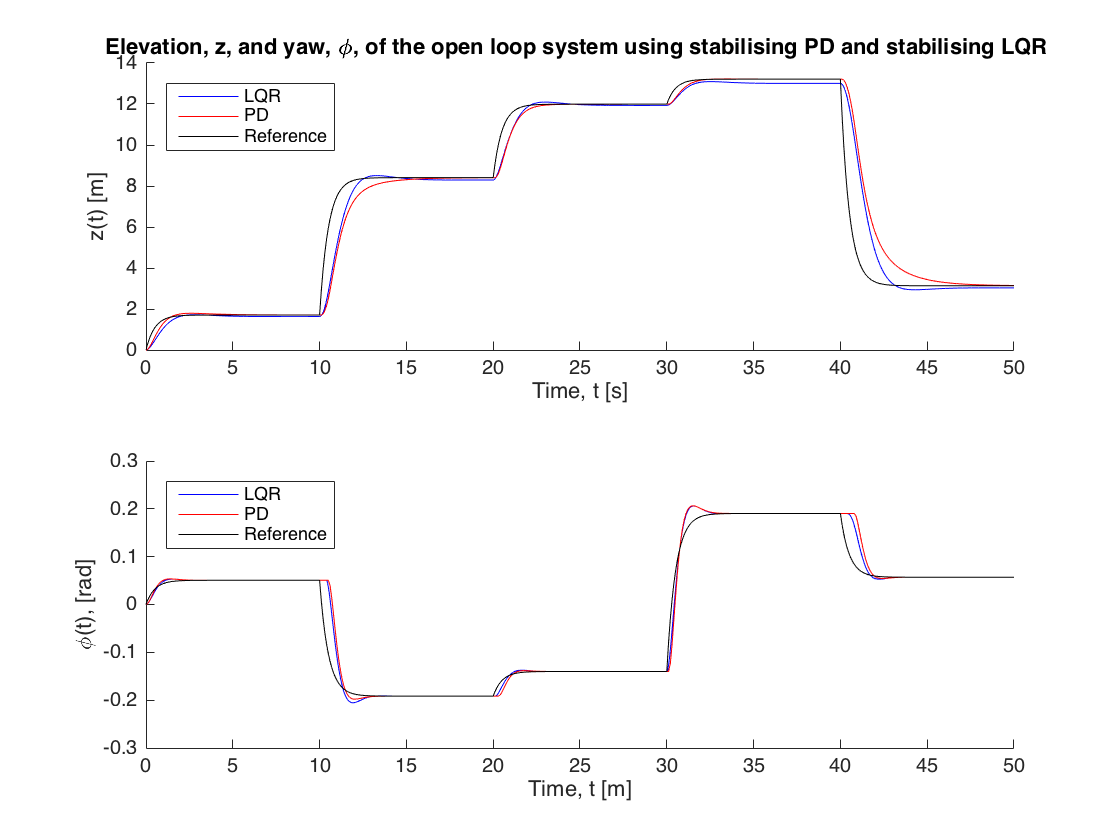
\includegraphics[width=0.8\textwidth]{figures/LQR-PD-comp.png}
\rule{35em}{0.5pt}
\caption{Comparision between the stabilising LQR- and PD-controllers.}
\label{fig:LQR-PD-comp}
\end{figure}

TODO: Write out the augmented linearised system matrices used in MPC.

\subsection{Rotor-loop dynamics}
TODO: Find transfer function from motor current to rotor speed on the form
\begin{equation}
H_{I\rightarrow \dot{\omega}}(s) \approx \frac{b_0}{s + a_0}
\end{equation}
The step response of the system is then
\begin{equation}
\frac{b_0}{s + a_0} \frac{1}{s} = \frac{b_0}{a_0}\Big(\frac{1}{s} - \frac{1}{s + a_0}\Big) \overset{\mathcal{L}_t}{\longrightarrow}
\frac{b_0}{a_0}(e^{-t} - e^{-a_0t})
\end{equation}
where the coefficients can be found with a regression. A simple test would be to measure the response of two unit steps in succession to determine both coefficients but for the purposes of simualtion, a rough estimate would be $a_0=40$ and $b_0 \approx 40*\omega_{max}/I_{max}$, which mathces the specification $||{\boldsymbol\omega}||_{\infty} \approx 0$ to $||{\boldsymbol\omega}||_{\infty} \approx 2.5\cdot 10^4$ in $< 180$ ms (see https://www.bitcraze.io/2015/02/measuring-propeller-rpm-part-3/). Here, $\omega_{max}$ is the maximum rotor speed of the quadcopter and $I_{max}\approx 1100$ mA is the peak motor current.

\section{State estimation}
To estimate the states properly, many approaches are considered and compared in simulation. The first is a regular Kalman filter (KF) which used the dynamics linearised around the stable hovering state to compute the filter gain ~\cite{glad2000control}. The second is an extended kalman filter (EKF), which effectively linearises the system around the previous state estimate on each time step. This is done by computing an expression for the Jacobian offline, which is then evaluated on-line, putting great constraints on how fast the inner loop can be run. In contrast to the KF, the EKF provides much better estimates when the system is far from the hovering state but it's not an optimal estimator.

\subsection{Unscented kalman filter}
The regular Kalman filter equations are omitted for brevity, but the EKF is implemented using the system representation
\begin{flalign}
\begin{split}
\mathbf{x}_{k+1} =& \mathbf{F}(\mathbf{x}_k,\mathbf{u}_k,\mathbf{v}_{k+1})\\
\mathbf{y}_{k} =& \mathbf{H}(\mathbf{x}_k,\mathbf{e}_{k+1})
\end{split}
\end{flalign}
The prediction step is then
\begin{flalign}
\begin{split}
\hat{\mathbf{x}}_{k}^- = & \mathbf{F}(\hat{\mathbf{x}}_{k-1},\mathbf{u}_{k-1}, \mathbf{v})\\
\mathbf{P}_{k}^-= & \mathbf{J}^F_{k-1}\mathbf{P}_{k-1} \mathbf{J}^F_{k-1} + \mathbf{Q}
\end{split}
\end{flalign}
based on the system dynamics, and a corrector step,
\begin{flalign}
\begin{split}
\mathbf{K}_{k} =& \mathbf{P}_{k}^-(\mathbf{J}^H_k)^T(\mathbf{J}^H_k \mathbf{P}_{k}^-(\mathbf{J}^H_k)^T + \mathbf{R})^{-1}\\
\hat{\mathbf{x}}_{k} =& \hat{\mathbf{x}}_{k}^- + \mathbf{K}_k(\mathbf{y_k} -\mathbf{H}(\mathbf{x}^-_k,\mathbf{e}))\\
\mathbf{P}_k =& (\mathbb{I} - \mathbf{K}_k\mathbf{J}^H_k)\mathbf{P}_{k}^-
\end{split}
\end{flalign}
where
\begin{equation}
\mathbf{J}^F_k = \frac{\partial \mathbf{F}(\mathbf{x}, \mathbf{u}_k, \mathbf{v})}{\partial \mathbf{x}}\Big|_{\mathbf{x}_k}
\qquad
\mathbf{J}^H_k = \frac{\partial \mathbf{H}(\mathbf{x}, \mathbf{e})}{\partial \mathbf{x}}\Big|_{\mathbf{x}_k}.
\end{equation}
In our implementation, $\mathbf{J}^F_k$ is stored as a symbolic expression and then evaluated on each iteration. The $\mathbf{H(x,e)}$ is a linear function and can therefore be replaced by $\mathbf{C}_d$ in ~\eqref{eq:continuoussys}.
\begin{figure}[htbp]
\centering
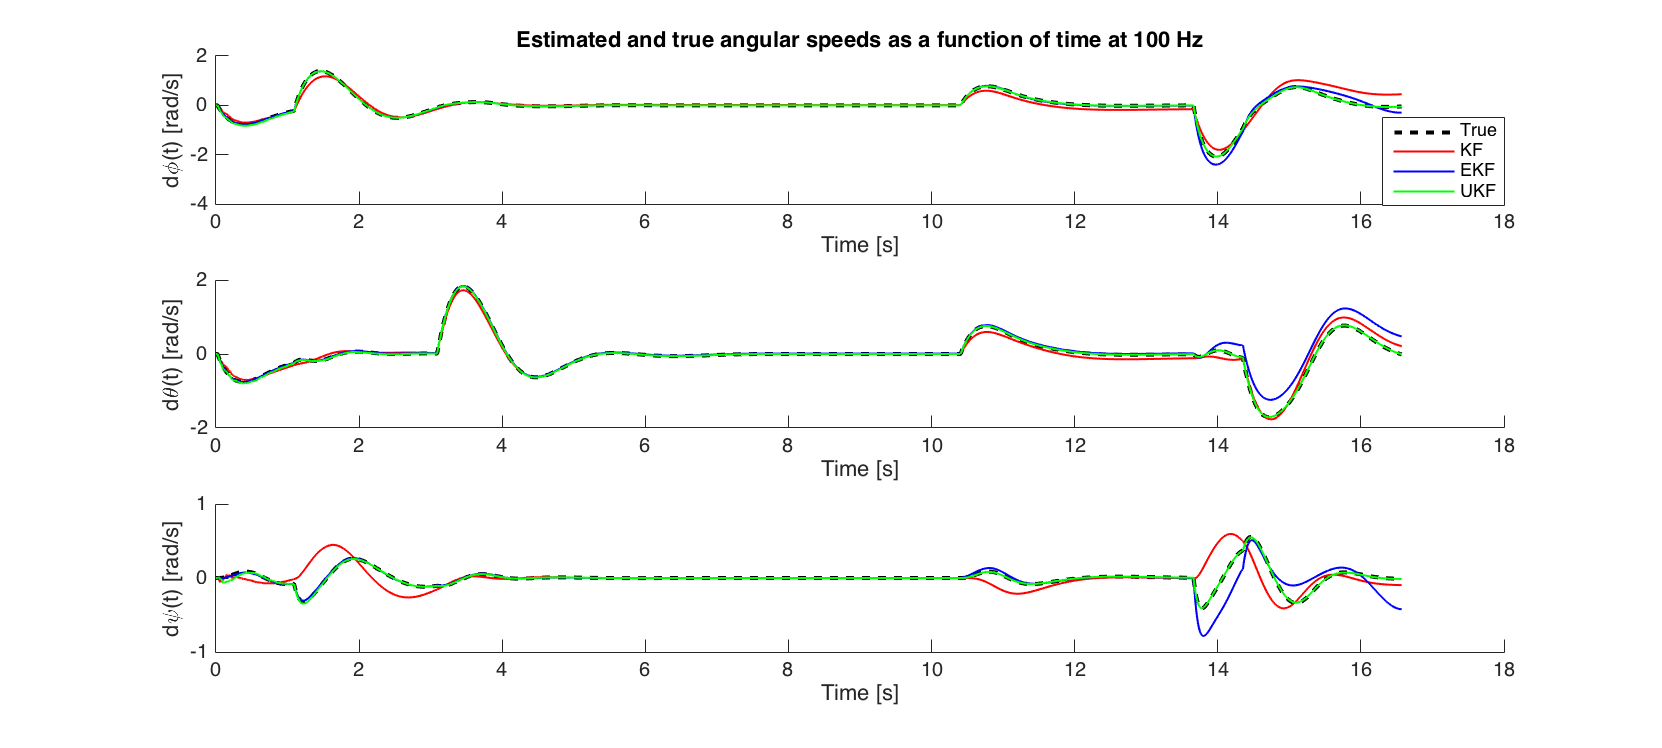
\includegraphics[width=1\textwidth]{figures/KalmanFilterComparison.png}
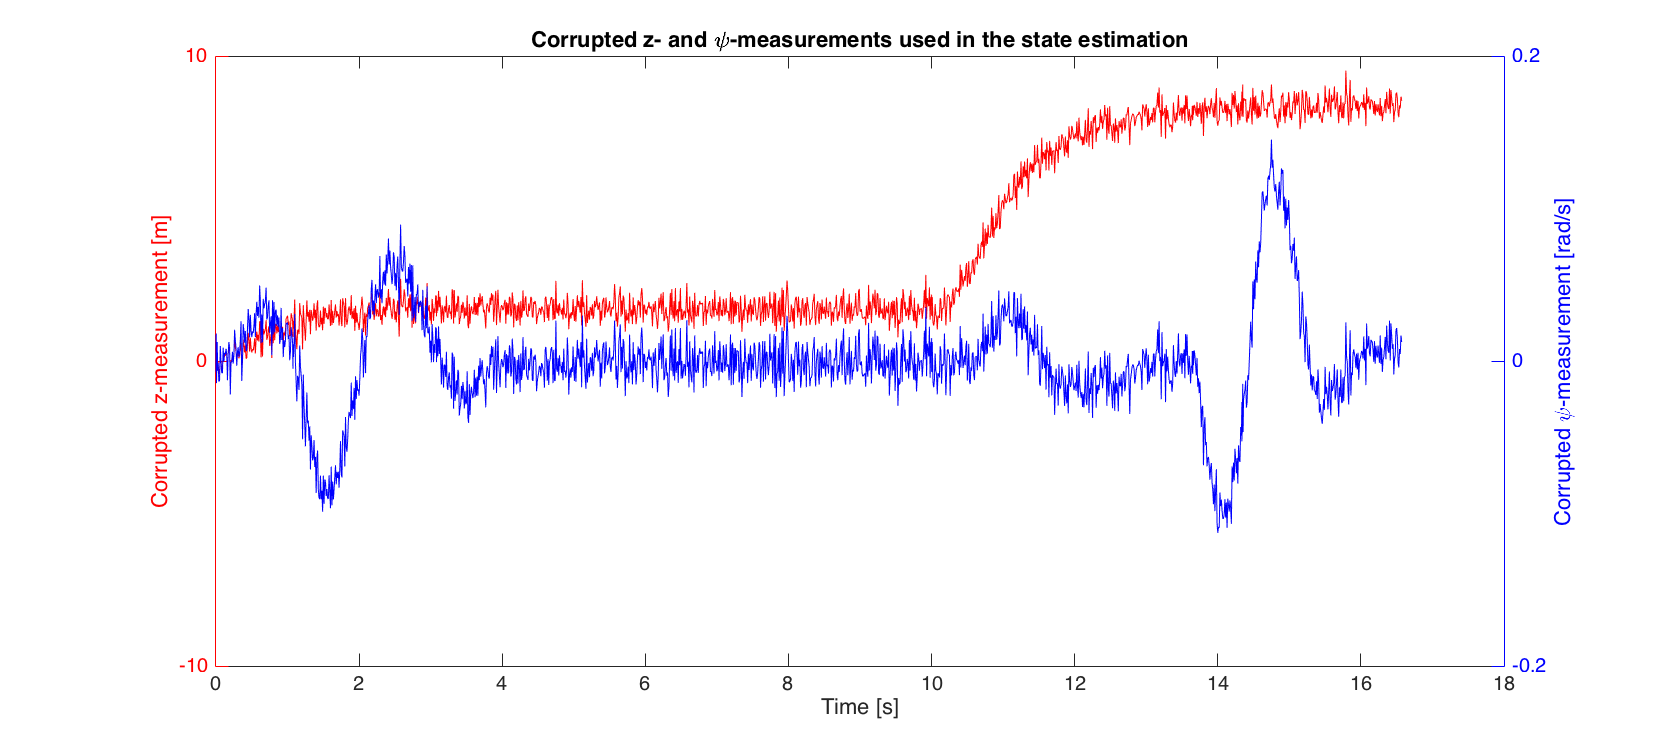
\includegraphics[width=1\textwidth]{figures/KalmanCompMeasurements.png}
\rule{35em}{0.5pt}
\caption{Demonstration of the drawbacks in using a regular Kalman compared to the EKF when estimating an unknown $\dot{\boldsymbol\eta}_k$, using (i) the same parameters in both filters (ii) having $\dot{\boldsymbol\eta}_k$ unknown and using (iii) corrupted measurements of $\boldsymbol\xi, \dot{\boldsymbol\xi}_k, \boldsymbol\eta_k$.}
\label{fig:KF-EKF}
\end{figure}

\subsection{Unscented kalman filter}
Attempted to implement the UKF (see algorithm 1 on page 4 in ~\cite{wan2000unscented}).

TODO: Write about unscented kalman ...

\subsection{Particle filter}
Attempted to implement the generic particle filter (see algorithm 3 on page 8 in ~\cite{arulampalam2002tutorial}). To combat degeneracy in the filter the systematic resampling is implemented due to it's simplicity and performance when compared to e.g. multinomial resampling~\cite{douc2005comparison}~\cite{hol2006resampling}.

TODO: Find out why the state amplitude becomes so small after resampling.

\subsection{Filter comparison}
An implementation of both all mentioned filters was made in Simulink as S-functions to allow the use of nestled- and external .m-functions (see *\texttt{/kalman\_filters/}). A double integrator with linear dynamics was set up to demonstrate the filters and how they are incorporated into a simulink model (see *\texttt{/Examples/double\_integrator\_filter\_test/}). The KFparam struct used to describe the filter is general enough to run an implemented filter in any application by simply defining the system and the necessary filter parameters, and is loaded from the *\texttt{\_init}-file. 

The filters were then applied and tested on nonlinear quadcopter dynamics, running with an inner stabilising PD loop at 100 Hz and a PID position controller at 50 Hz in the outer loop (see *\texttt{/Examples/inner\_loop\_filter\_test/}). To test performance, measurements of $\boldsymbol\xi_k, \dot{\boldsymbol\xi}_k, \boldsymbol\eta_k$ was corrupted with gaussian zero-mean uncorrelated noise with a variance of $\approx 0.3$ [m] on the positional states ($\boldsymbol\xi_k$), a variance of $0.1$ [m/s] on the velocities ($\dot{\boldsymbol\xi}_k$) and a variance of 0.01 on the Euler angles ($\dot{\boldsymbol\xi}_k$). The angular velocities were completely omitted and the process noise was assumed to be $\mathbf{0}$ at all times.

When running the example, the state estimation model block can be set with a filter by selecting one of the models in *\texttt{/kalman\_filters}. Which states to measure and design parameters are specified in the \texttt{init\_filters\_example.m} file, and resulting in the following estimation of the unknown angular velocities, $\dot{\boldsymbol\eta}_k$  (see Figure~\ref{fig:KF-EKF}). The regular kalman filter performs badly when the system is far from the stable states, and the over all error if is visibly larger in the KF. However, simulating the system at an inner loop sample rate of 100 Hz, the EKF is demands so much processing power that it becomes infeasible to implement in the physical process (unless other methods of computing the Jacobian are considered). In addition, the EKF estimation becomes more unstable as the step size increases, and already at a sample period of $T_s = 0.01 s$, the estimation becomes very poor after $\approx 16 s$ and the covariance matrix requires resetting (at higher sample rates such as 500 Hz, the filter performs well for an entire simulation duration of 50 s). The UKF has to be set with a fairly high $\alpha\approx0.5$ in order to spread the sigma points enough to properly capture the non-linear dynamics. It is far more economical in terms of computational power than the EKF and follows the true values much more accurately than any of the previously tested filters. This is clear when looking at the the error metric 
\begin{equation}
E(\mathbf{x},\hat{\mathbf{x}}) = \sum^{3}_i\int_0^{t_s} |\dot{\boldsymbol{\eta}}_i(t) - \dot{\hat{\boldsymbol{\eta}}}_i(t)|dt
\end{equation}
for the the estimation of the unknown states during a simulation time $t_s = 17$ [s]. Here, $E_{KF} \approx 4.2768$, $E_{EKF} \approx2.4781$, $E_{UKF} \approx0.1990$ showing that for this specific problem, the UKF the the better alternative in terms of accuracy and computational power (compared to the EKF).
 
\section{Motion planning}\label{sec:reftraj}
In this part of the project, we consider the polynomial generation method advanced by Roy et.al. cite XX. The general method is presented to make the Matlab code coherent, using the same nomenclature as in the code. The idea is to set up a constrained QP problem and solve it using Matlab's \texttt{quadprog} to find a minimum snap trajectory. The code will later be rewritten in Python/ROS with CVXGEN, and additional constraints will be enforced to ensure that the trajectory always stay in safe convex regions of space. These regions can conceivably be computed using IRIS, but will be assumed to be known initially.

Let the trajectory be composed of $n$ polynomials $P_{1}(t),...,P_{n}(t)$, where
\begin{equation}
P_{k}(t) = \sum\limits_{i = 0}^N p_it^i, \qquad t\in[0,T_k]
\end{equation}
with a maximum degree of $\deg(P_{k})=N$, and a corresponding coefficient vector $\mathbf{p}_{(k)}=[p_{k,0},...,p_{k,N}]$. The problem is then to minimise a cost function for every polynomial spline
\begin{equation}
J(T_k) = \int_0^{T_k} c_0P_{k}(t)^2 +  c_1P^{\prime}_k(t)^2  + ... + c_NP^{(N)}_{k}(t)^2 dt = \mathbf{p}_{(k)}^T\mathbf{Q}_{(k)}\mathbf{p}_k
\end{equation}
such that continuity is preserved and boundary conditions are enforced. In cite XX, the hessian matrix corresponding to a polynomial was derived by differentiating the term in the cost function containing the $r^{th}$ derivative of $P_{(k)}(t)$ with regards to the polynomial coefficients $p_i$, i.e. finding
\begin{equation}
\mathbf{Q}_{r,(k)}= \frac{\partial^2}{\partial p_i\partial p_j} \int_0^{T_k} P_{k}^{(r)}(t)^2dt
\end{equation}
and constructing the matrix
\begin{equation}
\mathbf{Q}_{(k)}=\mathbf{Q}_{(k)} = \sum\limits_{r = 0}^N c_r\mathbf{Q}_{r,(k)}\in \mathbb{R}^{(N+1)\times (N+1)}
\end{equation}
The complete constrained QP-formulation, including all $n$ polynomials is then
\begin{equation}
\text{Minimize}\Big(\sum_{k=1}^nJ(T_k)\Big)\qquad\text{subject to}\qquad\mathbf{A}\mathbf{p}-\mathbf{b}=0
\end{equation}
where
\begin{equation}
\end{equation}
\begin{equation}
\sum_{k=1}^nJ(T_k) =
\begin{bmatrix}
\mathbf{p}_{(1)} & \cdots & \mathbf{p}_{(n)}
\end{bmatrix}
\begin{bmatrix}
\mathbf{Q}_{(1)} & 0 & 0 \\
0 & \ddots & 0 \\
0 & 0 & \mathbf{Q}_{(n)}
\end{bmatrix}
\begin{bmatrix}
\mathbf{p}_{(1)} \\ \vdots \\ \mathbf{p}_{(n)}
\end{bmatrix}
 = \mathbf{p}^T\mathbf{Q}\mathbf{p}.
\end{equation}
For the $k^{th}$ polynomial, the $r^{th}$ derivative can be written
\begin{equation}
P_k^{(r)}(t) = \sum_{n=r}^N\Big(\prod_{m=0}^{r-1}(n-m)\Big)p_{k,n}t^{n-r}.
\end{equation}
Using this formula, boundary conditions can be enforced for each spline by finding a matrix 
\begin{equation}
\mathbf{A}_{(k)}
\mathbf{p}_{(k)} = 
\mathbf{b}_{(k)}
\end{equation}
for every know derivative at the time $t=0$ (collected in $\mathbf{A}_0$) and time $t=T_k$ (collected in $\mathbf{A}_T$). With $n_c$ boundary conditions for the $k^{th}$ spline, then
\begin{equation}
\mathbf{A}_{(k)} = 
\begin{bmatrix}\mathbf{A}_{0,k}\\
\mathbf{A}_{T,k}
\end{bmatrix}\in\mathbb{R}^{n_c\times N+1}
\quad\text{and}\quad
\mathbf{b}_{(k)} = 
\begin{bmatrix}\mathbf{b}_{0,k}\\
\mathbf{b}_{T,k}
\end{bmatrix}\in\mathbb{R}^{n_c\times1}
\end{equation}
For the remaining, free boundary endpoints where no fixed derivative is specified, the splines on each side of a boundary point are set equal by enforcing
\begin{equation}\label{eq:cont}
\mathbf{A}_{T,k}\mathbf{p}_k - \mathbf{A}_{0,k+1}\mathbf{p}_{k+1}=0.
\end{equation}
A general method of generating the $\mathbf{Q}$- and $\mathbf{A}$-matrices was implemented in matlab (see \texttt{get\_Q}, \texttt{get\_A}), called by the \texttt{compute\_splines} method which used \texttt{quadprog}'s interior point method to find a solution given a set of points, times and a cost vector. This, and the demo script \texttt{splines\_2\_1D\_example.m} is located in the /crazy\_trajectory directory and is almost in a good state. The problem can be solved using various polynomial degrees and finds connecting splines, but the continuity conditions in free points~\label{eq:cont} is still not working properly (see Figure~\ref{fig:splines}). Clearly, the jerk squared is minimised and the the polynomial splines are continuos, but the derivatives are not. We have yet to figure out why.
\begin{figure}[htbp]
\centering
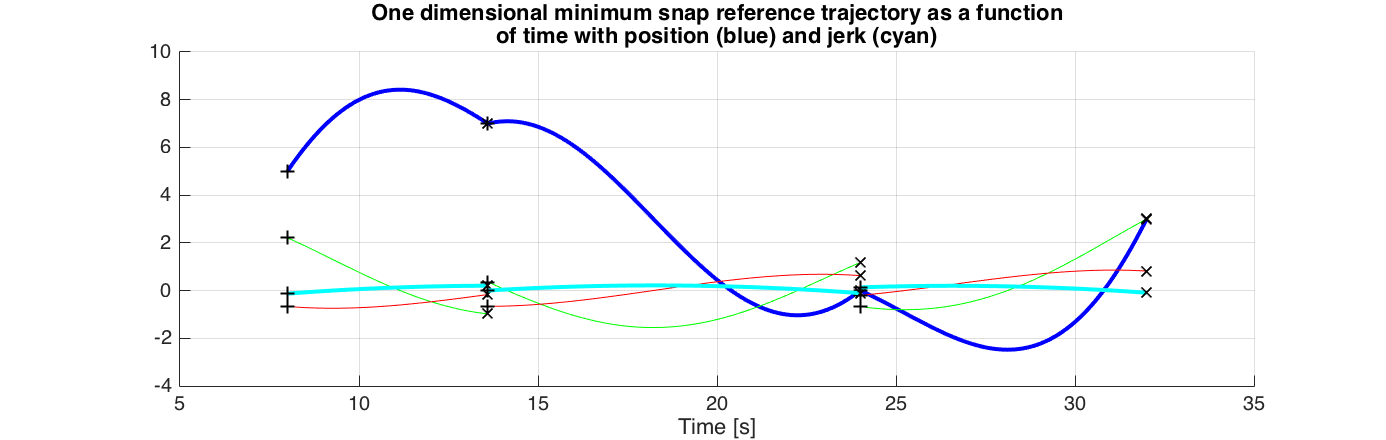
\includegraphics[width=0.8\textwidth]{figures/Splines.png}
\rule{35em}{0.5pt}
\caption{A reference trajectory composed of three splines with a maximum order of $N = 5$ and cost vector $c = [0,0,0,1,0,0]$ (minimum snap), enforcing positional endpoint conditions and at unevenly spaced times, with $t = [8,13.6,24,32]$.}
\label{fig:splines}
\end{figure}

\section{Reference tracking LQR with feedforward term}
In this section, we the PD augmented linearised state-space model in discrete time and include integrated states
\begin{equation}
\mathbf{x}_{e} = \begin{bmatrix}\mathbf{x}\\\mathbf{z}\end{bmatrix}
\mathbf{A}_{e} = []
\end{equation}

o solve the associated Ricatti equation for 
\section{MPC control}
For the MPC control, the system dynamics is augmented with stabilising PD control in \textbf{Section \ref{sec:PD}}, and linearised around a stable point. The system was implemented in Matlab without state estimation using the MPC-tools 1.0 developed at LTH cite XX as a proof of concept (see \texttt{/Examples/quadcopter\_mpc\_position\_test.slx}). The result was equivalent to that of the PID-PD controller when using a fixed reference point for all states on the prediction horizon, and can be expected to improved if using time-varying reference generated in the motion planning. As the MPC-tools solution is (i) incredibly slow, (ii) unable to handle varying references on the prediction horizon and (iii) not apt for a Python/C-realtime implementation in ROS, alternatives were investigated. The two candidates are CVXgen and QPgen, which both generate fast QP solvers in C, and can be set up to suffice (i).

The MPC-problem formulation, with a time varying reference, $\mathbf{r}_k$, and a control signal, $\mathbf{u}_k$, kept close to the angular velocity required to hover, $\mathbf{u}^s$, can be written
\begin{flalign}
\begin{split}
\min\Big(\sum^{m}_{k=1}(\mathbf{x}_k - \mathbf{r} _k)^T\mathbf{Q}(\mathbf{x}_k - \mathbf{r} _k) + \sum^{n}_{k=1}(\mathbf{u}_k-\mathbf{u}^s)^T\mathbf{R}(\mathbf{u}_k-\mathbf{u}^s)\Big)\\
\mathbf{x}_{k + 1} = \mathbf{A}^d\mathbf{x}_k+ \mathbf{B}^d\mathbf{u}_k, \qquad k = 0,...,m\\
|\mathbf{x}_{7,k + 1}| < x_{max}, \qquad k = 1,...,m\\
|\mathbf{x}_{9,k + 1}| < x_{max}, \qquad k = 1,...,m\\
|\mathbf{u}_k - \mathbf{u}^s| < u_{max}, \qquad k = 1,...,n\\
||\mathbf{u}_{k} - \mathbf{u}_{k-1}||_{\infty} < S_{max}, \qquad k = 1,...,n\\
\end{split}.
\end{flalign}
Where $\mathbf{Q}\in\mathbb{R}^{10\times 10}_+, \mathbf{R}\in\mathbb{R}^{4\times 4}_+$ are diagonal cost matrices, $\mathbf{A}^d\in\mathbb{R}^{10\times 10}, \mathbf{B}^d\in\mathbb{R}^{10\times 4}$ are the ZOH-sampled, discrete time system matrices of the augmented state space model. The remaining constraints bound the pitch and yaw, bound the deviation in control signal from the linearisation point $\mathbf{u}^s$, and the final puts a hard constraint on how fast we allow the control signal to vary. This final constraint can be set very high or removed completely, as the motors are incredibly responsive.

With this formulation with $m,n = 10$, the QP solver generated by CVXgen has 5364 non-zero KKT entries, which is slightly above the recommended 4000. To evaluate the feasibility of the CVXgen solver with the above formulation, a Simulink implementation was made using the MEX-solver, replacing the MPC-tools solver with a rewritten S-function (see \texttt{MPC\_CVX.m}). The solver seems to work perfectly with the simulink environment, and is, as suspected, incredibly much faster than the already implemented \texttt{qp\_is.m} solver of the MPC-tools. The implementation is still not complete, and can presently only be run as an open loop system, where $\mathbf{u}_0$ is set to 

In order to use The MPC solver efficiently, the reference trajectory generated by the optimisation in \textbf{Section \ref{sec:reftraj}} has to be evaluated on the prediction horizon, i.e, at each cycle of the MPC-loop, we need to find a matrix $\mathbf{R}_{ref} = \begin{bmatrix}\mathbf{r}_1 & \cdots & \mathbf{r}_m\end{bmatrix}$, which evaluates the splines. The splines are in an array of polynomial coefficients, $\mathbf{P}$, defined on $t\in[t_0,t_f]$. Numerical evaluation needs to be done $m$ times at a period time of $T_s$, starting at the current time, $t_c$. Special caution needs to be taken if a sample time $t_k \neq [t_0,t_f]$, in which case the quadcopter is set to hover in the appropriate end of the trajectory.

For these purposes, the scripts \texttt{reftraj\_compute\_example.m} and \texttt{reftraj\_eval\_example.m} were written. The former computes a trajectory in space with fixed positions at certain points in time, the derivatives are left free and currently, there is an issue with continuity, as described in \textbf{Section \ref{sec:reftraj}}. The latter forms the $\mathbf{R}_{ref}$-matrix, and the resulting reference samples on the prediction horizon is plotted (see Figure~\ref{fig:trajectory}).
\begin{figure}[htbp]
\centering
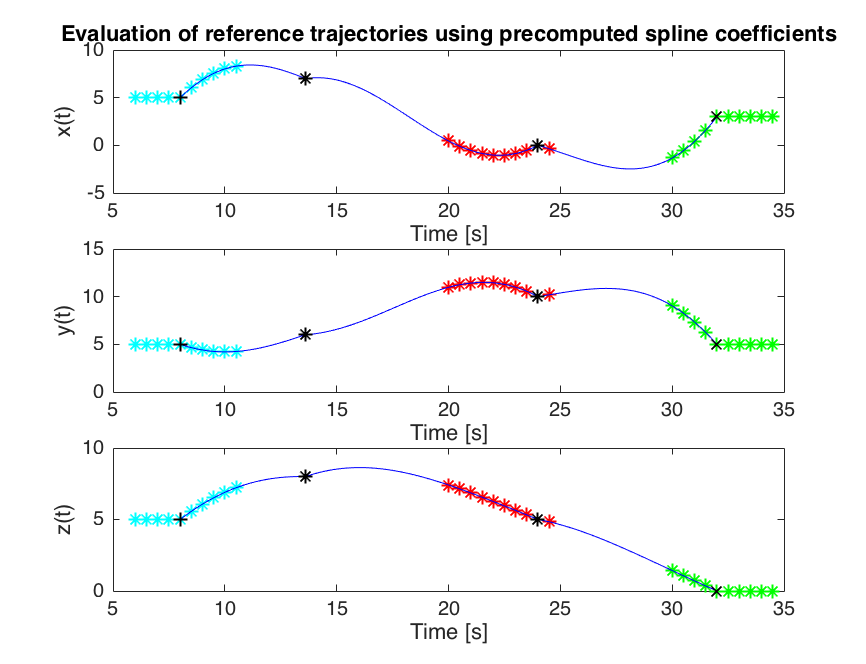
\includegraphics[width=0.5\textwidth]{figures/Trajectory.png}%
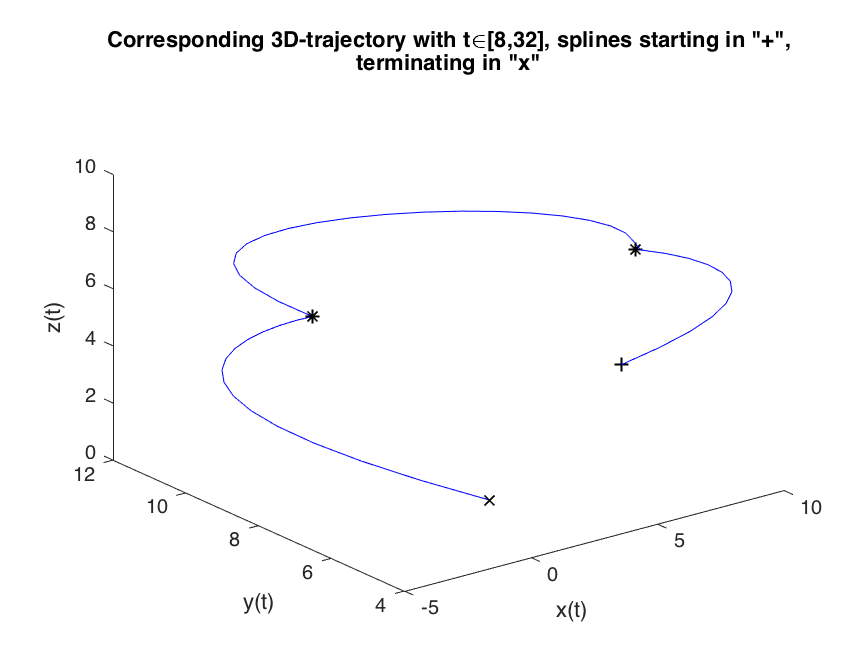
\includegraphics[width=0.5\textwidth]{figures/Trajectory3d.png}
\rule{35em}{0.5pt}
\caption{A reference trajectory composed of three 3D-splines with a maximum order of $N = 5$ and cost vector $c = [0,0,0,1,0,0]$ (minimum snap), enforcing positional endpoint conditions and at unevenly spaced times, with $t_0=8$ and $t_f=32$. The splines were evaluated with $T_s = 0.5$, $m = 10$, $t_c = 6\Rightarrow$ some $t_k < t_0$ (cyan), $t_c = 20\Rightarrow$ all $t_k\in[t_0,t_f]$ (red) and $t_c = 30\Rightarrow$ some $t_k > t_f$ (green). As can be seen, the algorithm properly evaluates the splines at evenly spaced times and makes the reference hover at a trajectory endpoint if $t_k\neq[t_0,t_f]$. Here, only the positional elements of $\mathbf{R}_{ref}$ are plotted, note the reference velocities and anles are also evaluated. }
\label{fig:trajectory}
\end{figure}

\subsubsection*{TODO}
\begin{enumerate}
\item \sout{Create simplified linearised system model for use in MPC} (see eg.~\cite{Bouffard:EECS-2012-241}).
\item \sout{Validate by comparison to the results in}~\cite{Bouffard:EECS-2012-241}.
\item \sout{Set up MPC controller with Simulink MPC-library} (see eg.~\cite{Bouffard:EECS-2012-241}).
\item \sout{Validate by comparison to the results in}~\cite{Bouffard:EECS-2012-241}.
\item Set up MPC controller with CVXgen and S-fucntions (see eg.~\cite{Bouffard:EECS-2012-241}~\cite{mattingley2012cvxgen}).
\item Validate by comparison to the results in Simulink.
\item System identification.
\item Simulate system with proper parameters.
\item Compare the four different implementations based on speed and stability.
\end{enumerate}

\section{$\mathcal{L}_1$-control}
Here we consider control of the linearized system
The $\mathbf{\Gamma}$-projection operator for two vectors $\theta,y\in\mathbb{R}^k$ is defined as
\begin{equation}
\text{Proj}_{\mathbf{\Gamma}}(\theta,y,f) =
\begin{cases}
\mathbf{\Gamma} y - \mathbf{\Gamma}\dfrac{\nabla f(\theta)(\nabla f(\theta))^T}{||\nabla f(\theta)||_2}\mathbf{\Gamma} yf(\theta)\qquad
\text{if}\;\;f(\theta)>0\;\;\text{and}\;\;y^T\nabla f(\theta)>0\\
\mathbf{\Gamma} y\qquad\qquad\qquad\qquad\qquad\qquad\quad\quad\text{otherwise}.
\end{cases}
\end{equation}
where $\mathbf{\Gamma} = \mathbb{I}_{k\times k}\Gamma$ for some scalar $\Gamma > 0$ (typically $\Gamma\approx 10^5$) and $f(\theta)$ is a convex function~\cite{lavretsky2011projection}. By solving the Lyapunov equation
\begin{equation}
\mathbf{A}_m\mathbf{X}+ \mathbf{X}\mathbf{A}_m^T+ \mathbf{Q} = 0,
\end{equation}
for $\mathbf{P}=\mathbf{P}^T$, with some arbitrary $\mathbf{Q}>0$, the feedback controller
\begin{equation}
\begin{cases}
u(t)=\hat{\theta}^Tx(t)+k_gr(t)\\
\dot{\hat{\theta}}(t) = \text{Proj}_{\mathbf{\Gamma}}(\hat{\theta}^T(t),x(t)\tilde{x}^T(t)\mathbf{X}b)
\end{cases}
\end{equation}
can be constructed, where $\tilde{x} = \hat{x} - x$ is the state estimation error, $k_g$ is a gain and $r(t)$ is the reference signal. By designing the companion system
\begin{equation}
\begin{cases}
\dot{x}(t) = \mathbf{A}_m\hat{x}(t) + b(u(t)-\hat{\theta}^T(t)x(t))\\
y(t) = c^T\hat{x}(t)
\end{cases}
\end{equation}
it can be shown (by Theorem 2~\cite{cao2006design}) that the state estimation error,
\begin{equation}
\lim_{t\rightarrow\infty}\tilde{x} = 0.
\end{equation}
By a corollary of the theorem, choosing
\begin{equation}
k_g =-\frac{1}{c^T\mathbf{A}_m^{-1}b} \Rightarrow \lim_{t\rightarrow\infty}y(t) = r
\end{equation}
if $r \equiv$ constant.
\begin{enumerate}
\subsubsection*{TODO}
\item \sout{Define general control structure.}
\item Create Simulink projection operator (see eg.~\cite{L1control})
\item Validate projection operator against benchmark Simulink models (eg. ~\cite{cao2006design}).
\item Define robustness metrics (see eg.~\cite{L1control}~\cite{huynh20141})
\item Create script for computing the $\mathcal{L}_1$-gain (see eg.~\cite{L1control}).
\item Validate script against benchmark Simulink models (eg. ~\cite{cao2006design}).
\item Simulate control.
\end{enumerate}

\section{ROS implemetation}
Wolfgang's crazyros driver~\cite{HoenigMixedReality2015}

\begin{figure}[htbp]
\centering
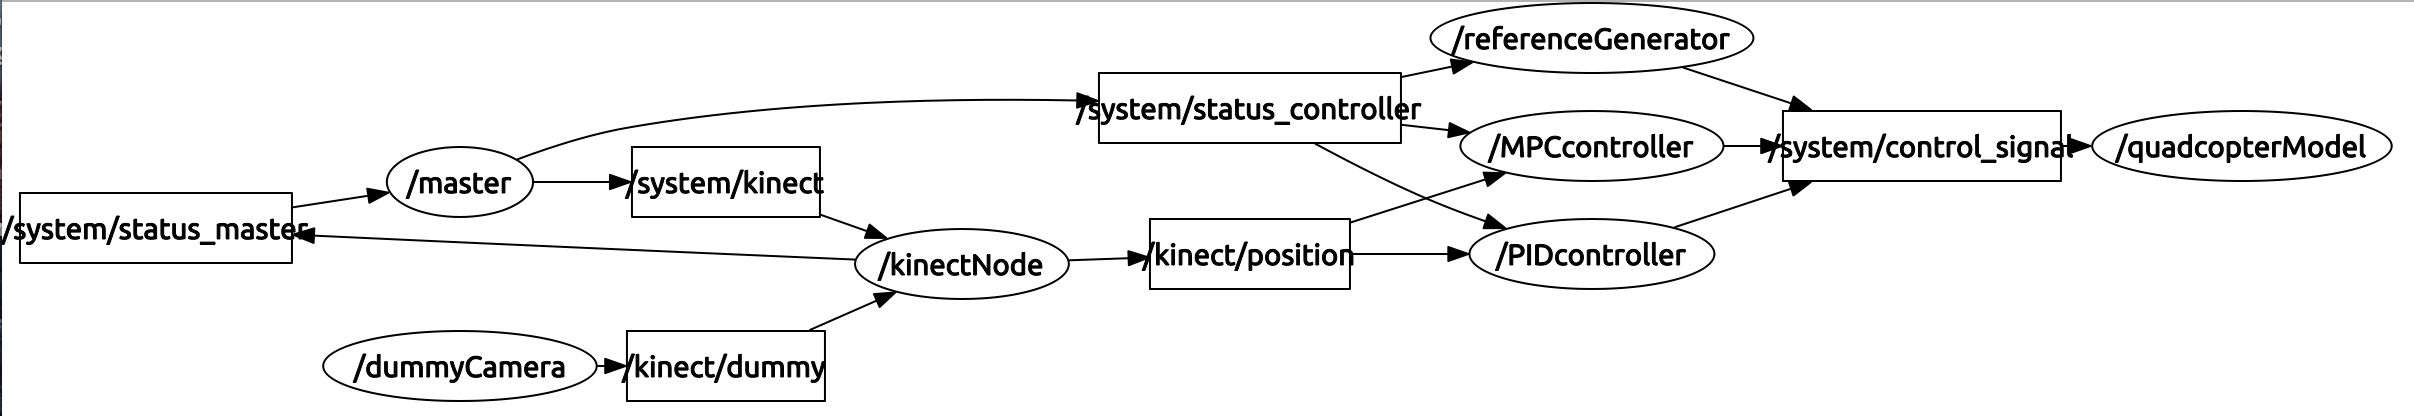
\includegraphics[width=\textwidth,trim={1mm 0 0 0.7mm},clip]{figures/ROSstruct.png}
\rule{35em}{0.5pt}
\caption{The current ROS structure as generated in \texttt{rqt\_plot} with nodes (ellipses), topics (boxes) and the connecting arrows intdicating the flow of information.}
\label{fig:ROSstruct}
\end{figure}
\subsection{Kinect node}
The kinect node subscribes to the /camera/depth/image\_rect-topic, to which the ``openni'' software publishes information in the data type ``Image'', which is part of the standard ROS messages library ``sensor\_msgs''. This node handles the raw camera data and publishes the quadcopter position to the topic /kinect\_pos\_measurement as a 3x1 float 64 numpy array. The reason for this choice of data type is to enable realt time plotting of the position with rviz and rqt\_plot.

The camera is calibrated by taking 100 consecutive samples of the background noise, from which a mean depth is computed. 
When running, the measured depth matrix is subtracted with the background noise so that only a handful of pixels are zero separate (or rather above some threshold $\epsilon\approx 2$ depth units). This set of pixels, $S$, is then used to compute the depth of the copter as the mean of the depths of all pixels in $S$. Similarity, the quadcopter position in the image is computed as the mean of all x and y pixel indices of the points in $S$.

The angle of the camera is calibrated by taking a set of $N$ measurement points, $\mathbf{p}_i=\begin{bmatrix}x_i,y_i,z_i\end{bmatrix}$, in the background depth matrix. From these points, the center of mass is computed as
\begin{equation}
\bar{\mathbf{p}}= \begin{bmatrix}\bar{x},\bar{y},\bar{z}\end{bmatrix} = \frac{1}{N}\sum_{i = 1}^N \mathbf{p}_i,
\end{equation}
and a matrix for each point's deviation from the center of mass is set up
\begin{equation}
\mathbf{P} = \begin{bmatrix}\mathbf{p}_1\\ \vdots \\ \mathbf{p}_N\end{bmatrix} -  \begin{bmatrix}\bar{\mathbf{p}}\\ \vdots \\ \bar{\mathbf{p}}\end{bmatrix}\in\mathbb{R}^{N\times 3},
\end{equation}
The matrix $\mathbf{P}$ is then factorised using the singlar value decomposition (SVD), from which, the left-singular vector corresponding to the smallest of the three singular values is the normal of the best fitting plane in a least-squares sense, $\bar{\mathbf{n}}_{xyz}$. As we are only interested in the angle $\alpha$ in the $xz$-plane, the normal is projected onto this plane, resulting in the normal $\bar{\mathbf{n}}_{xz}$ (see Figure~\ref{fig:planecalibration}). From this, the angle is simply computed using the cosine dot product definition
\begin{equation}
\alpha = \arccos\Big(\frac{\bar{\mathbf{n}}_{xz}\cdot \hat{\mathbf{x}}_c}{||\bar{\mathbf{n}}_{xz}||_2}\Big).
\end{equation}

\begin{figure}[htbp]
\centering
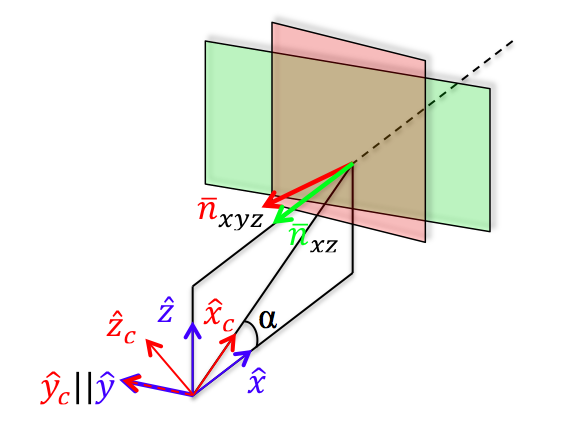
\includegraphics[width=0.5\textwidth]{figures/kinectcal.png}
\rule{35em}{0.5pt}
\caption{.}
\label{fig:planecalibration}
\end{figure}

Once the angle has been computed, we are ready to detect moving objects. By subtracting the background data from each measured image and computing the center of mass of all the points in $S$, we get an estimate of the quadcopter's center of mass in terms of depth and pixel indices. This point is then mapped into the camera coordinate system [m], where the depth unit is mapped to a distance from the camera to the quadcopter [m] by an exponential function, and the aperture of the camera is used to translate the position of the copter to a point in space in the camera coordinate system, $\mathbf{p}_c$, with origin at the camera. This point is then translated into the global coordinate system, $\mathbf{p}$, (in which the controller operates) by means of the transformation
\begin{equation}
\mathbf{p} = \begin{bmatrix} \cos(\alpha)& 0 & -\sin(\alpha) \\ 0 & 1 & 0 \\ \sin(\alpha) & 0 & \cos(\alpha)\end{bmatrix} \mathbf{p}_c.
\end{equation}

\section{General TODOs}
\begin{enumerate}
\item Found that one of the copters were broken - sent to Bitcraze for repairs, expected to be done in early march.
\item Tried installing IRIS in Ubuntu but ran into issues using the PODS "make" command required to get everything up and running. TODO: contact Claes or Anders to get help in finding someone experienced with PODS.
\end{enumerate}

\newpage\bibliography{bibliography}{}
\bibliographystyle{IEEEtran}

\section{Appendix}\label{sec:appendix}
\end{document}